\section{calibrate.c File Reference}
\label{calibrate_8c}\index{calibrate.c@{calibrate.c}}
{\tt \#include $<$msp430x16x.h$>$}\par
{\tt \#include $<$stdio.h$>$}\par
{\tt \#include $<$stdlib.h$>$}\par
{\tt \#include $<$signal.h$>$}\par
{\tt \#include \char`\"{}ueaclib.h\char`\"{}}\par
{\tt \#include \char`\"{}ueac.h\char`\"{}}\par
{\tt \#include \char`\"{}calibrate.h\char`\"{}}\par
{\tt \#include \char`\"{}conversion.h\char`\"{}}\par
{\tt \#include \char`\"{}timer.h\char`\"{}}\par
{\tt \#include \char`\"{}filter.h\char`\"{}}\par
{\tt \#include \char`\"{}global.h\char`\"{}}\par
{\tt \#include \char`\"{}external\_\-flash.h\char`\"{}}\par


Include dependency graph for calibrate.c:\begin{figure}[H]
\begin{center}
\leavevmode
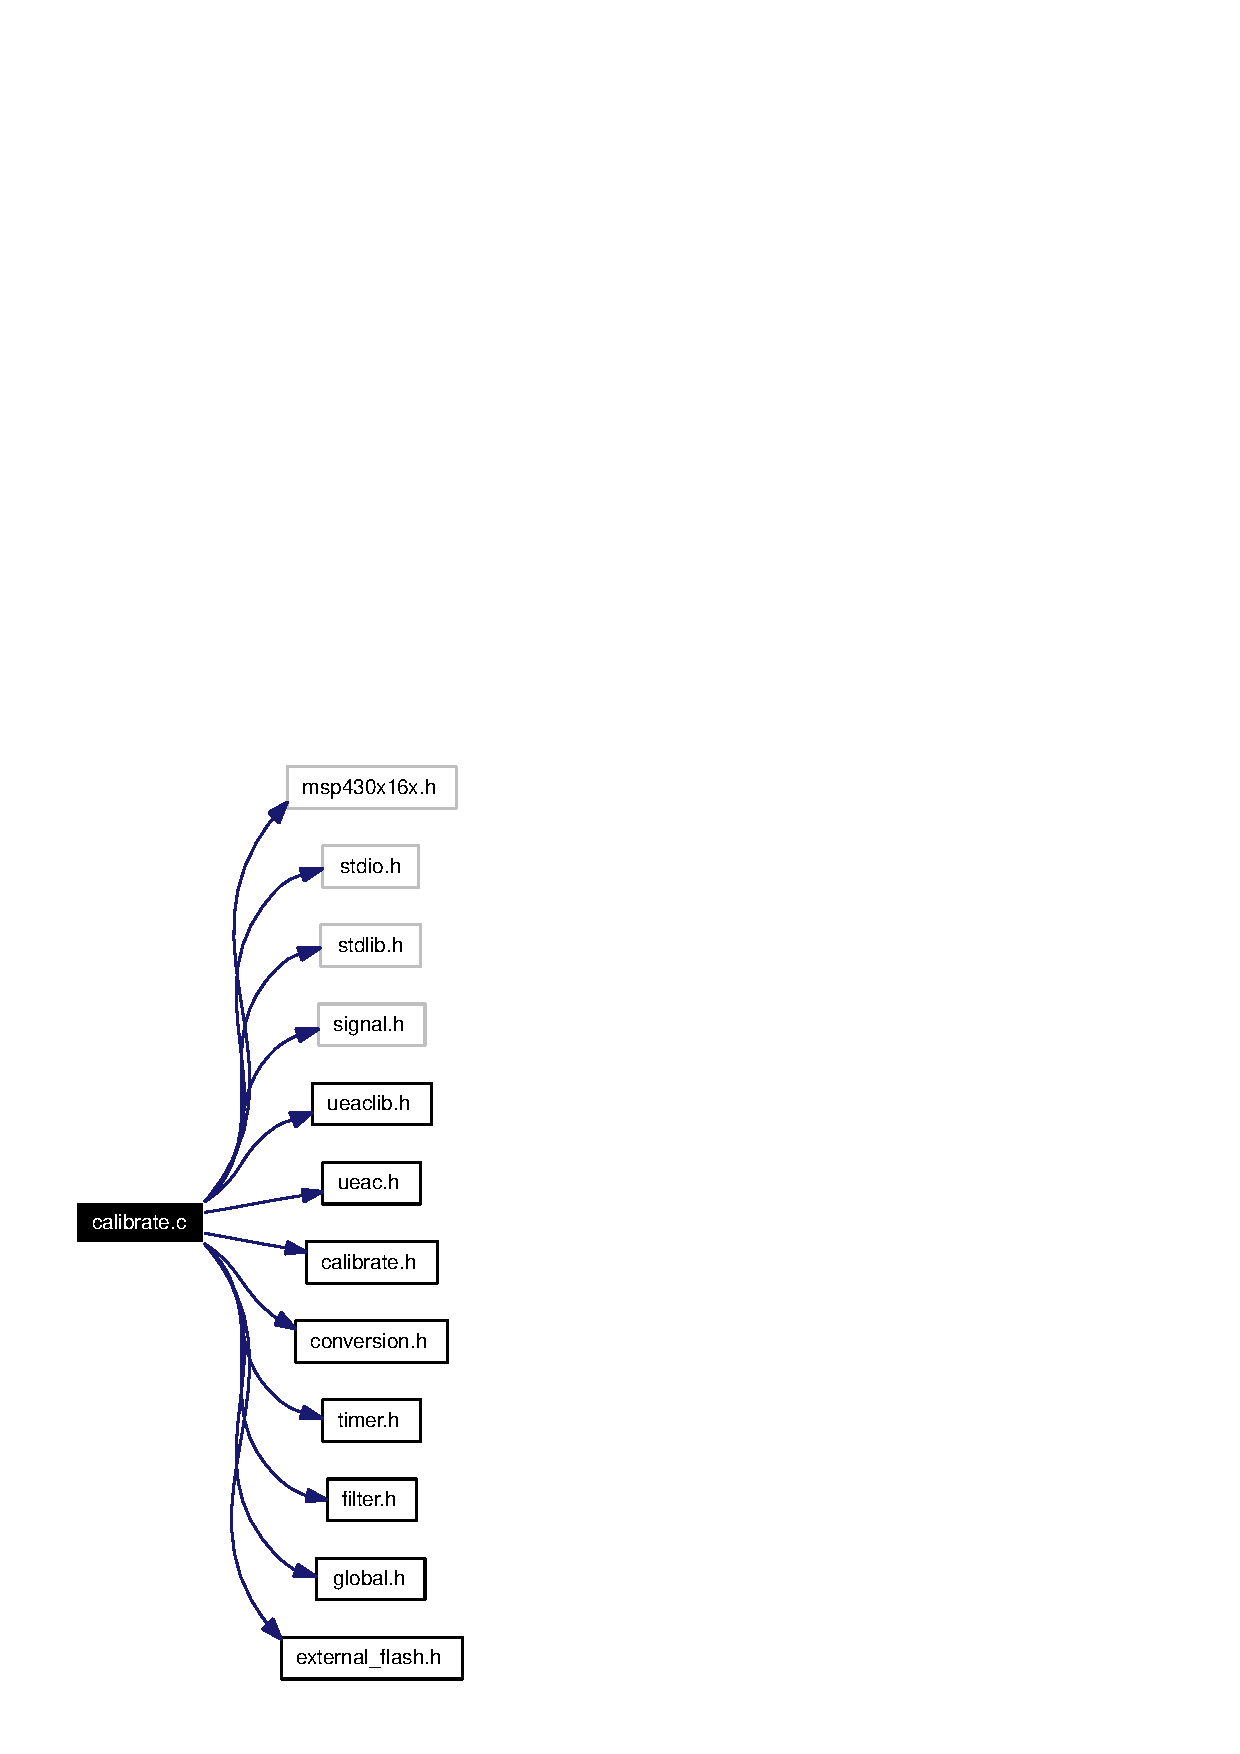
\includegraphics[width=111pt]{calibrate_8c__incl}
\end{center}
\end{figure}
\subsection*{Defines}
\begin{CompactItemize}
\item 
\#define {\bf LED\_\-DWELL}~100
\end{CompactItemize}
\subsection*{Functions}
\begin{CompactItemize}
\item 
void {\bf scan\_\-leds} (void)
\item 
void {\bf current\_\-output\_\-calibration} ({\bf ueac\_\-t} $\ast$system)
\item 
void {\bf current\_\-input\_\-calibration} ({\bf ueac\_\-t} $\ast$system)
\item 
void {\bf voltage\_\-input\_\-calibration} ({\bf ueac\_\-t} $\ast$system)
\end{CompactItemize}
\subsection*{Variables}
\begin{CompactItemize}
\item 
short {\bf dac\_\-translation} [$\,$]
\end{CompactItemize}


\subsection{Define Documentation}
\index{calibrate.c@{calibrate.c}!LED_DWELL@{LED\_\-DWELL}}
\index{LED_DWELL@{LED\_\-DWELL}!calibrate.c@{calibrate.c}}
\subsubsection{\setlength{\rightskip}{0pt plus 5cm}\#define LED\_\-DWELL~100}\label{calibrate_8c_a0}




Definition at line 58 of file calibrate.c.

Referenced by scan\_\-leds().

\subsection{Function Documentation}
\index{calibrate.c@{calibrate.c}!current_input_calibration@{current\_\-input\_\-calibration}}
\index{current_input_calibration@{current\_\-input\_\-calibration}!calibrate.c@{calibrate.c}}
\subsubsection{\setlength{\rightskip}{0pt plus 5cm}void current\_\-input\_\-calibration ({\bf ueac\_\-t} $\ast$ {\em system})}\label{calibrate_8c_a4}




Definition at line 248 of file calibrate.c.

\footnotesize\begin{verbatim}248                                                 {
249   printf("\n\rCurrent Input Calibration\n\r");
250 }
\end{verbatim}\normalsize 


\index{calibrate.c@{calibrate.c}!current_output_calibration@{current\_\-output\_\-calibration}}
\index{current_output_calibration@{current\_\-output\_\-calibration}!calibrate.c@{calibrate.c}}
\subsubsection{\setlength{\rightskip}{0pt plus 5cm}void current\_\-output\_\-calibration ({\bf ueac\_\-t} $\ast$ {\em system})}\label{calibrate_8c_a3}




Definition at line 111 of file calibrate.c.

References buffer1\_\-to\_\-page\_\-e(), buffer1\_\-write(), convert\_\-a2d(), dac\_\-translation, delay\_\-1\_\-25m\-S(), getchar(), cal::i\_\-200u\-A\_\-offset, I\_\-CONVERSION, cal::i\_\-zero\_\-offset, ueacval::integer, PAGE\_\-SIZE, ueac::pin\_\-cal, pin\_\-data, write\_\-current(), write\_\-dac(), write\_\-led(), and write\_\-lla().

Referenced by ueac\_\-execute\_\-instruction().

\footnotesize\begin{verbatim}111                                                  {
112   enum {FIND_ESCAPE,FIND_LEFT_BRACKET,EVALUATE_ARROW};
113   int i;
114   char ch;
115   int parse_state=FIND_ESCAPE;
116   int i_offset=0;
117   int found=0;
118   int sum,current;
119   ueacval_t result;
120 
121 
122   printf("\n\rCurrent Output Calibration\n\r");
123   printf("Attach the DVM in current mode to the pin with the active LED\n\r");
124   printf("Use the up arrow and down arrow keys to adjust the current\n\r");
125   printf("-----------------------------------------------------------------\n\r");
126   buffer1_write(0,'V');        // write the valid char to the first location of external flash                          
127   for (i=1;i<PAGE_SIZE;i++) {  // clear out the external flash's SRAM buffer
128     buffer1_write(i,0);
129   }
130   for (i=0;i<25;i++) {
131     write_lla(i,0);
132     write_led(i,1);
133     found=0;
134     i_offset=0;
135     printf("%d@200uA> ",i);
136     while (!found) {
137       write_dac(i,dac_translation[0]+i_offset);  
138       if (((ch=getchar())!='\n')&&(ch!='\r')) {
139         switch (parse_state) {
140         case FIND_ESCAPE:
141           if (ch==0x1b) {
142             parse_state=FIND_LEFT_BRACKET;
143           }
144           break;
145         case FIND_LEFT_BRACKET:
146           if (ch=='[') {
147             parse_state=EVALUATE_ARROW;
148           }
149           else {
150             parse_state=FIND_ESCAPE;
151           }
152           break;
153         case EVALUATE_ARROW: 
154           if (ch=='A') {
155             i_offset--;
156           }
157           else if (ch=='B') {
158             i_offset++;
159           }
160           parse_state=FIND_ESCAPE;
161           break;
162         }
163       }
164       else {
165         buffer1_write(i+1,i_offset);
166         printf("%d\n\r",i_offset);
167         found=1;
168         system->pin_cal[i].i_200uA_offset=i_offset;
169       }
170     }
171     found=0;
172     i_offset=0;
173     printf("%d@0uA> ",i);
174     while (!found) {
175       write_dac(i,dac_translation[200]+i_offset);  
176       if (((ch=getchar())!='\n')&&(ch!='\r')) {
177         switch (parse_state) {
178         case FIND_ESCAPE:
179           if (ch==0x1b) {
180             parse_state=FIND_LEFT_BRACKET;
181           }
182           break;
183         case FIND_LEFT_BRACKET:
184           if (ch=='[') {
185             parse_state=EVALUATE_ARROW;
186           }
187           else {
188             parse_state=FIND_ESCAPE;
189           }
190           break;
191         case EVALUATE_ARROW: 
192           if (ch=='A') {
193             i_offset--;
194           }
195           else if (ch=='B') {
196             i_offset++;
197           }
198           parse_state=FIND_ESCAPE;
199           break;
200         }
201       }
202       else {
203         buffer1_write(i+26,i_offset);
204         printf("%d %d\n\r",i_offset,dac_translation[200]+i_offset);
205         found=1;
206         system->pin_cal[i].i_zero_offset=i_offset;
207       }
208     }
209     write_led(i,0);
210   }
211   for (i=0;i<25;i++) {
212     write_lla(i,1);
213     printf("%d ",i);
214     sum=0;
215     for (current=200;current>0;current-=50) {
216       write_current(i,current);
217       delay_1_25mS(500);
218       convert_a2d(I_CONVERSION,pin_data[i].filtered_result,&result,25);
219       printf("%d ",result.integer);
220       sum+=(current-result.integer);
221     }
222     write_current(i,0);
223     delay_1_25mS(500);
224     convert_a2d(I_CONVERSION,pin_data[i].filtered_result,&result,25);
225     printf("floor=%d,",result.integer);
226     buffer1_write(i+51,result.integer);
227     printf("offset=%d\n\r",sum/4);
228     buffer1_write(i+76,sum/4);
229     write_lla(i,0);
230   }
231   printf("Commit calibration to external flash ? (y or n) ");
232   while (1) {
233     if (((ch=getchar())=='y')||(ch=='Y')) {
234       buffer1_to_page_e(0);
235       printf("\n\rCalibration Saved !\n\r");
236       break;
237     }
238     if ((ch=='n')||(ch=='N')) {
239       printf("\n\rCalibration Abort !\n\r");
240       break;
241     }
242     else {
243       printf("\n\rPlease respond with y or n: ");
244     }
245   }
246 }
\end{verbatim}\normalsize 




Here is the call graph for this function:\begin{figure}[H]
\begin{center}
\leavevmode
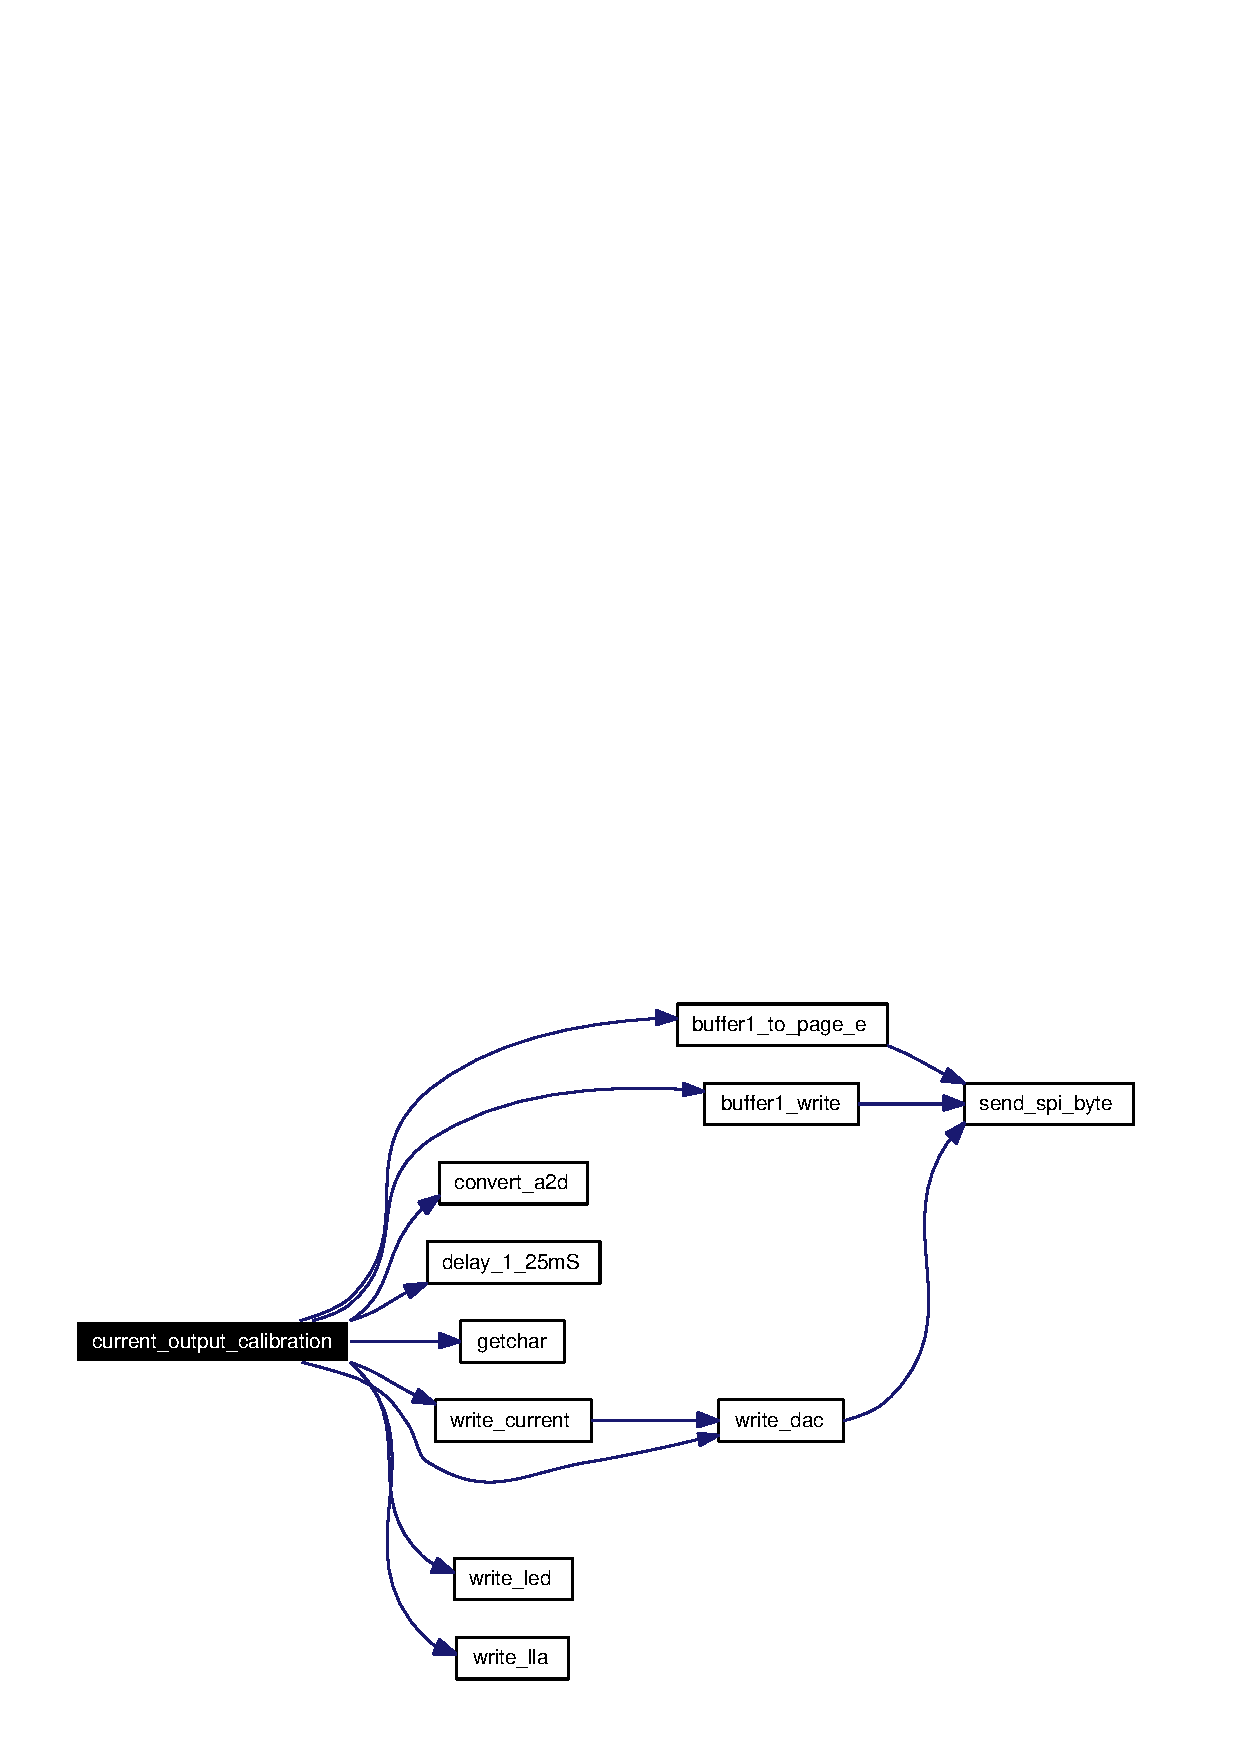
\includegraphics[width=272pt]{calibrate_8c_a3_cgraph}
\end{center}
\end{figure}
\index{calibrate.c@{calibrate.c}!scan_leds@{scan\_\-leds}}
\index{scan_leds@{scan\_\-leds}!calibrate.c@{calibrate.c}}
\subsubsection{\setlength{\rightskip}{0pt plus 5cm}void scan\_\-leds (void)}\label{calibrate_8c_a2}




Definition at line 61 of file calibrate.c.

References BLACK, delay\_\-1\_\-25m\-S(), GREEN, LED\_\-DWELL, and write\_\-led().

Referenced by main().

\footnotesize\begin{verbatim}61                      {
62   enum {OFF,ON};
63   int index; 
64   printf("Scanning LEDs ");
65   // All LEDs off
66   for (index=0;index<25;index++) {
67     write_led(index,OFF);
68   }
69   // Scan Rows 
70   for (index=0;index<25;index+=5) {
71     write_led(index,ON);
72     write_led(index+1,ON);
73     write_led(index+2,ON);
74     write_led(index+3,ON);
75     write_led(index+4,ON);
76     delay_1_25mS(LED_DWELL);
77     write_led(index,OFF);
78     write_led(index+1,OFF);
79     write_led(index+2,OFF);
80     write_led(index+3,OFF);
81     write_led(index+4,OFF);
82   }
83   // Scan Columns 
84   for (index=0;index<5;index++) {
85     write_led(index,ON);
86     write_led(index+5,ON);
87     write_led(index+10,ON);
88     write_led(index+15,ON);
89     write_led(index+20,ON);
90     delay_1_25mS(LED_DWELL);
91     write_led(index,OFF);
92     write_led(index+5,OFF);
93     write_led(index+10,OFF);
94     write_led(index+15,OFF);
95     write_led(index+20,OFF);
96   }
97   // All LEDs ON
98   for (index=0;index<25;index++) {
99     write_led(index,ON);
100   }
101   delay_1_25mS(LED_DWELL*2);
102   // All LEDs OFF
103   for (index=0;index<25;index++) {
104     write_led(index,OFF);
105   }
106   printf(GREEN);
107   printf("[DONE]\n\r");
108   printf(BLACK);
109 }
\end{verbatim}\normalsize 




Here is the call graph for this function:\begin{figure}[H]
\begin{center}
\leavevmode
\includegraphics[width=109pt]{calibrate_8c_a2_cgraph}
\end{center}
\end{figure}
\index{calibrate.c@{calibrate.c}!voltage_input_calibration@{voltage\_\-input\_\-calibration}}
\index{voltage_input_calibration@{voltage\_\-input\_\-calibration}!calibrate.c@{calibrate.c}}
\subsubsection{\setlength{\rightskip}{0pt plus 5cm}void voltage\_\-input\_\-calibration ({\bf ueac\_\-t} $\ast$ {\em system})}\label{calibrate_8c_a5}




Definition at line 252 of file calibrate.c.

\footnotesize\begin{verbatim}252                                                 {
253   printf("\n\rVoltage Input  Calibration\n\r");
254 }
\end{verbatim}\normalsize 




\subsection{Variable Documentation}
\index{calibrate.c@{calibrate.c}!dac_translation@{dac\_\-translation}}
\index{dac_translation@{dac\_\-translation}!calibrate.c@{calibrate.c}}
\subsubsection{\setlength{\rightskip}{0pt plus 5cm}short {\bf dac\_\-translation}[$\,$]}\label{calibrate_8c_a1}




Definition at line 45 of file cal\_\-table.h.